\documentclass[a4paper]{article}
\usepackage{amsmath,amssymb,caption,float,graphicx,xcolor}
\usepackage[utf8]{inputenc}
% \usepackage[english]{babel}
% \usepackage[backend=bibtex]{biblatex}
% \addbibresource{Lab3.bib}
\captionsetup[figure]{labelsep=period}
\captionsetup[table]{labelsep=period}
% \definecolor{bg}{rgb}{0.95,0.95,0.95}
\renewcommand\thesection{\arabic{section}}
% \usemintedstyle{emacs}
\begin{document}
\begin{center}
    \huge
    \textbf{ECE4730J\\Advanced Embedded System\\}
    \Large
    \vspace{15pt}
    \uppercase{\textbf{Lab 2: Program Profiling on Linux}}\\
    \large
    \vspace{5pt}\today\\
    \vspace{5pt}
    \begin{tabular}{ll}
        Name&Student ID\\
        Yihua Liu&518021910998\\
        Shuocheng Chen&517021911139\\
        Yiming Ju&518370910059\\
    \end{tabular}
    \vspace{5pt}
    \rule[-5pt]{.97\linewidth}{0.05em}
\end{center}
Lab 1 Task 3. (Optional)
\begin{figure}[H]
    \centering
    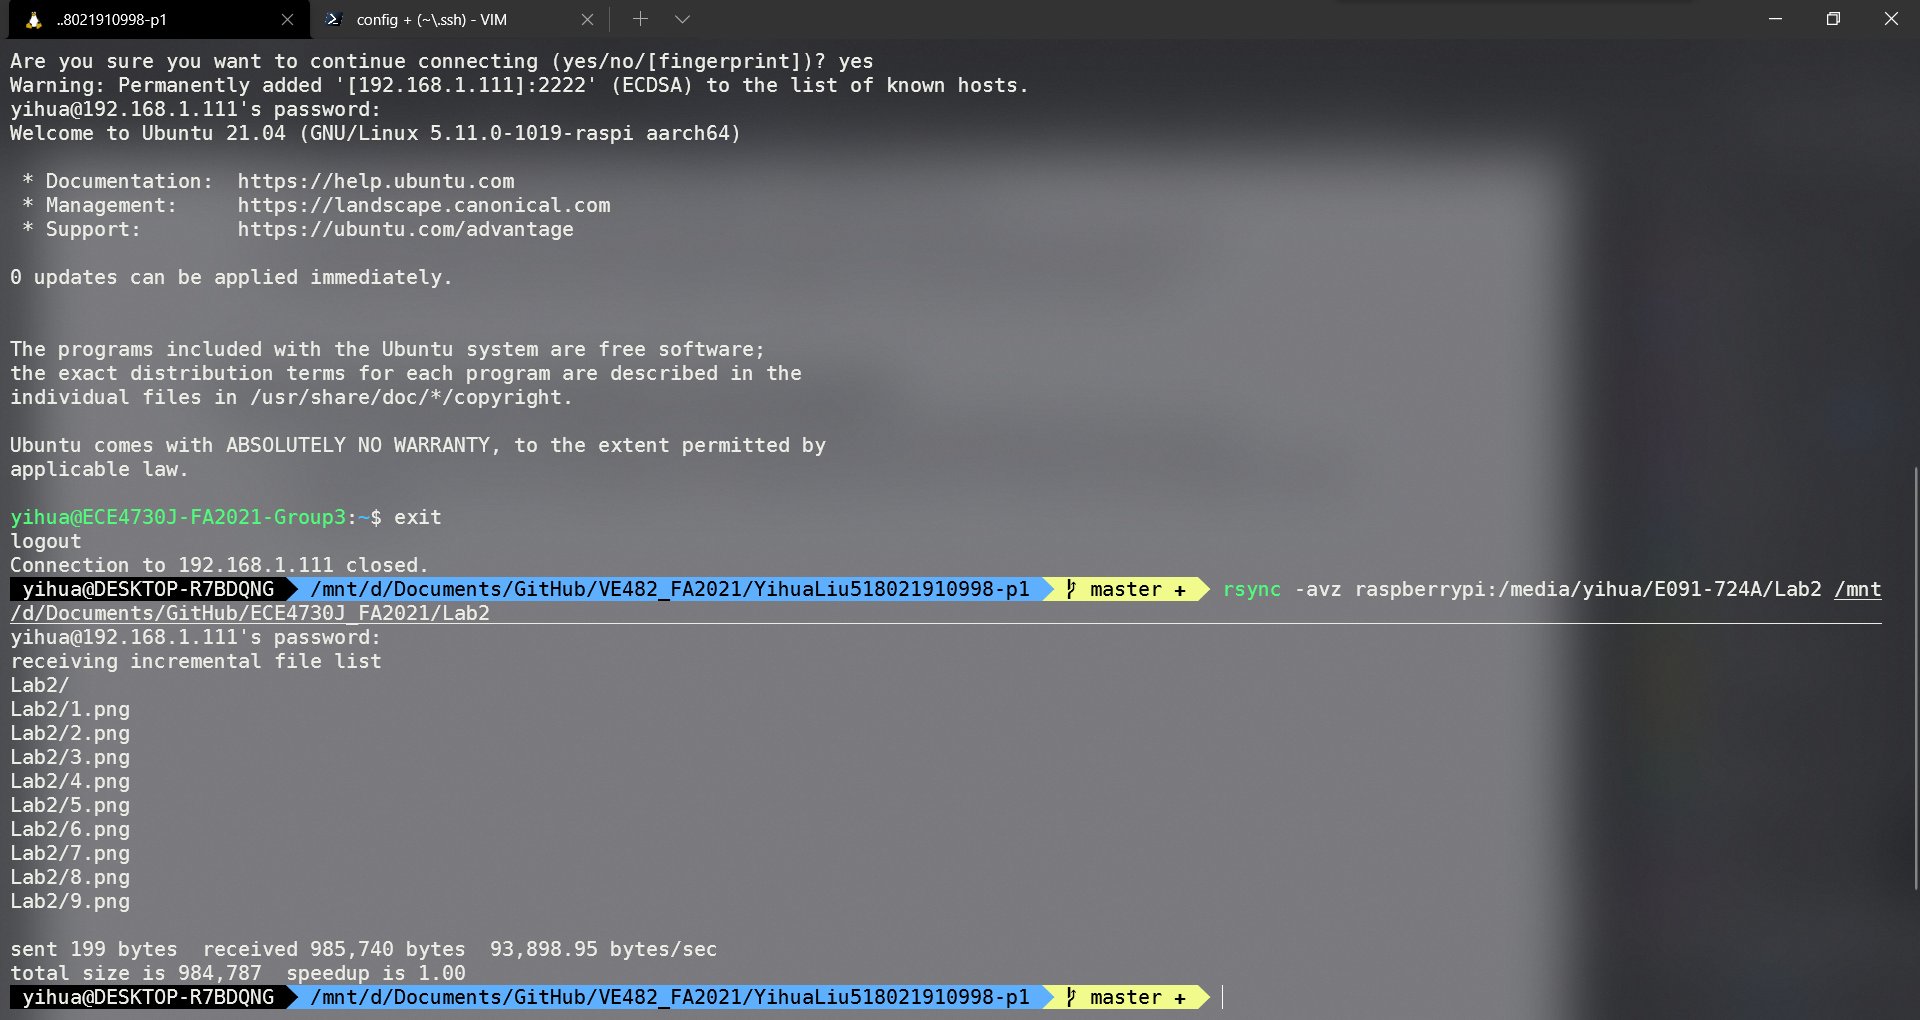
\includegraphics[width=1\textwidth]{0.png}
    \caption{Setup the remote access to your Raspberry Pi.}
\end{figure}
1. No submission for the first exercise.

2.
\begin{figure}[H]
    \centering
    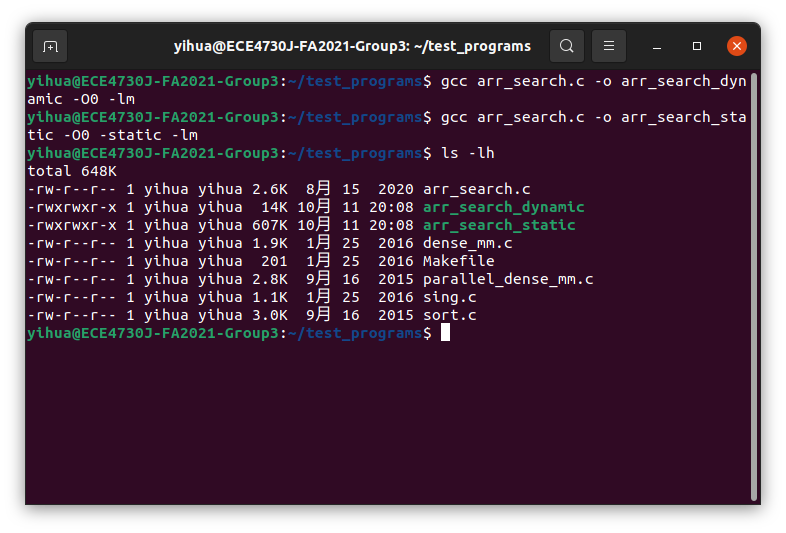
\includegraphics[width=1\textwidth]{1.png}
    \caption{The list of the size of each program.}
\end{figure}
\begin{table}[H]
    \centering
    \begin{tabular}{|c|c|}
        \hline
        program&size\\
        \hline
        arr\_search\_static&607K\\
        \hline
        arr\_search\_dynamic&14K\\
        \hline
    \end{tabular}
    \caption{The list of the size of each program.}
\end{table}
The statically compiled program is much larger than the dynamically compiled program because the statically compiled program includes all the library code in the executable file, while the dynamically compiled program places calls to the code of shared libraries during runtime.

3.
\begin{figure}[H]
    \centering
    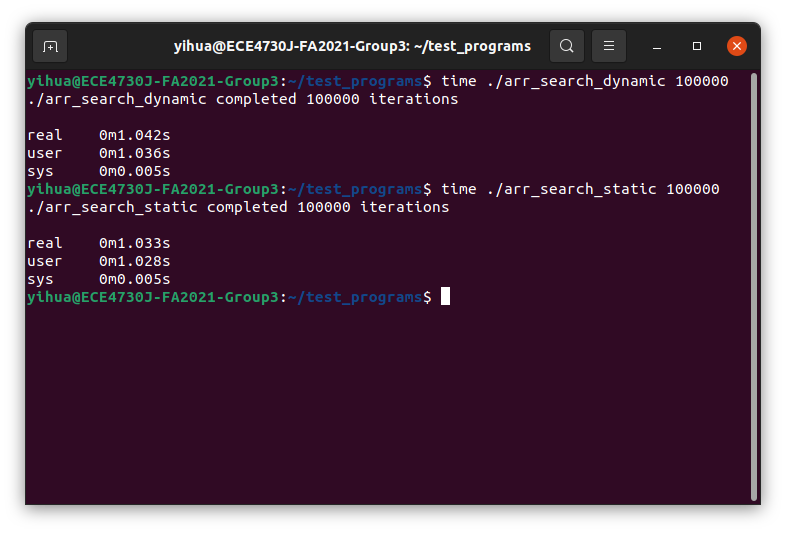
\includegraphics[width=1\textwidth]{2.png}
    \caption{\texttt{time} command.}
\end{figure}
The number of iterations used: 100000.

Note that there should be enough time interval between two measures of time, otherwise the measurement will be inaccurate.

The "real" execution time for the arr\_search\_dynamic binary: 1.042s.

The "real" execution time for the arr\_search\_static binary: 1.033s

The statically compiled program is slightly faster than the dynamically compiled program because the statically compiled program can directly execute the library code without calling to shared library. However, the difference is very small. If you repeat many times, you will find that sometimes they almost have the same execution time.

4.
\begin{figure}[H]
    \centering
    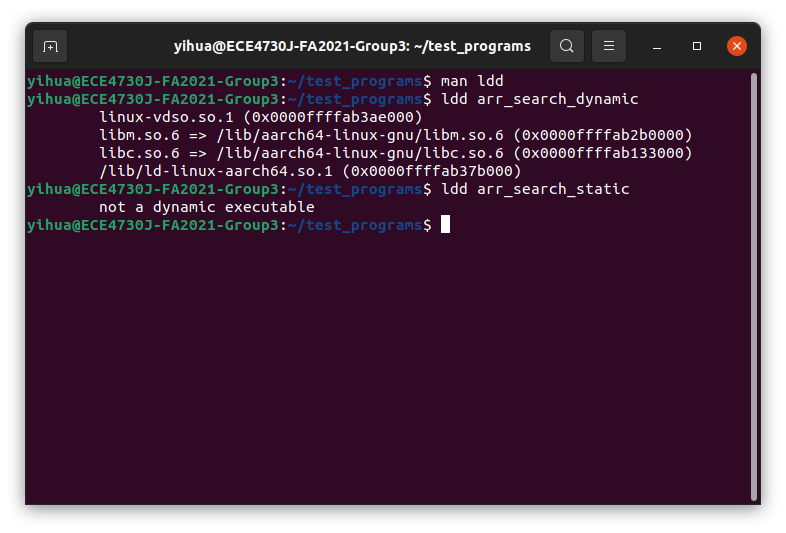
\includegraphics[width=1\textwidth]{3.png}
    \caption{\texttt{ldd} command.}
\end{figure}
They are different because \texttt{ldd} is used to print shared object dependencies. The statically compiled program does not require shared objects (shared libraries), so it prompts "not a dynamic executable". On the contrary, the dynamically compiled program requires shared objects (shared libraries), so \texttt{ldd} prints the shared objects (shared libraries) it used:\\
linux-vdso.so.1\\
libm.so.6 =\textgreater /lib/aarch64-linux-gnu/libm.so.6\\
libc.so.6 =\textgreater /lib/aarch64-linux-gnu/libc.so.6\\
/lib/ld-linux-aarch64.so.1

5.
\begin{figure}[H]
    \centering
    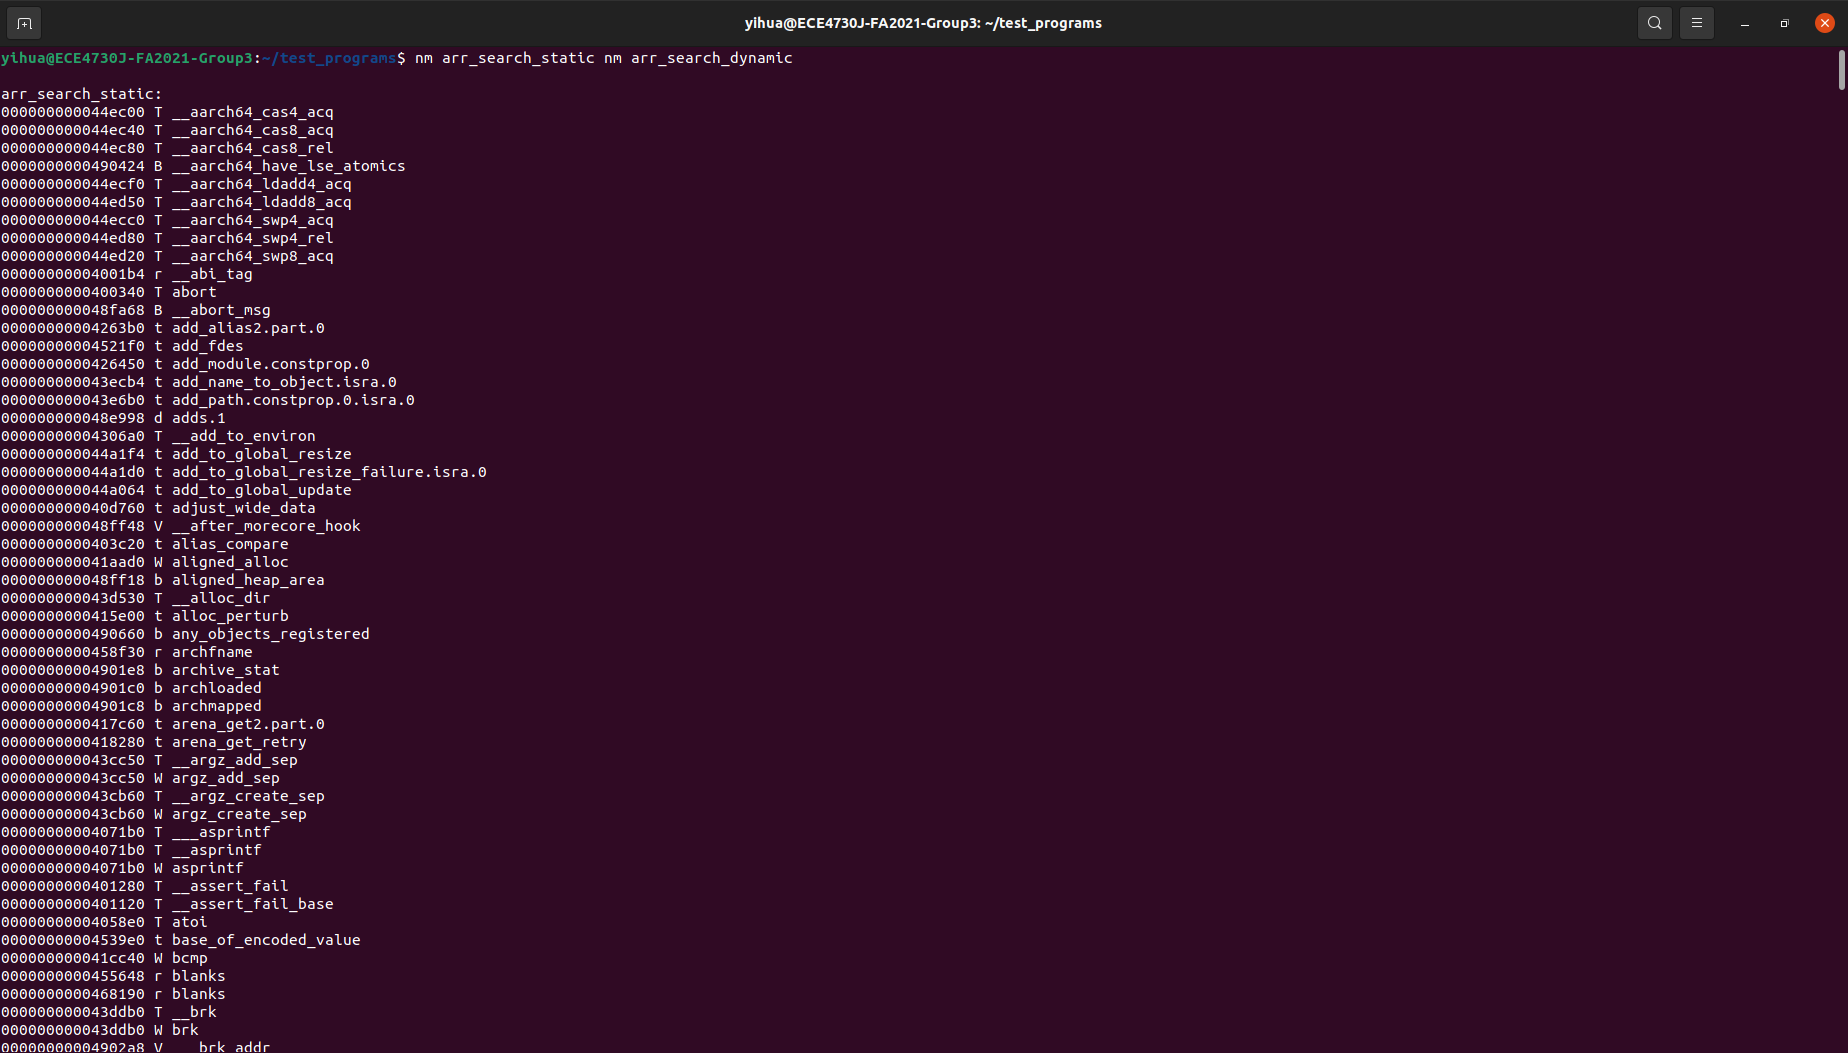
\includegraphics[width=1\textwidth]{4.png}
    \caption{\texttt{nm} command (static).}
\end{figure}
\begin{figure}[H]
    \centering
    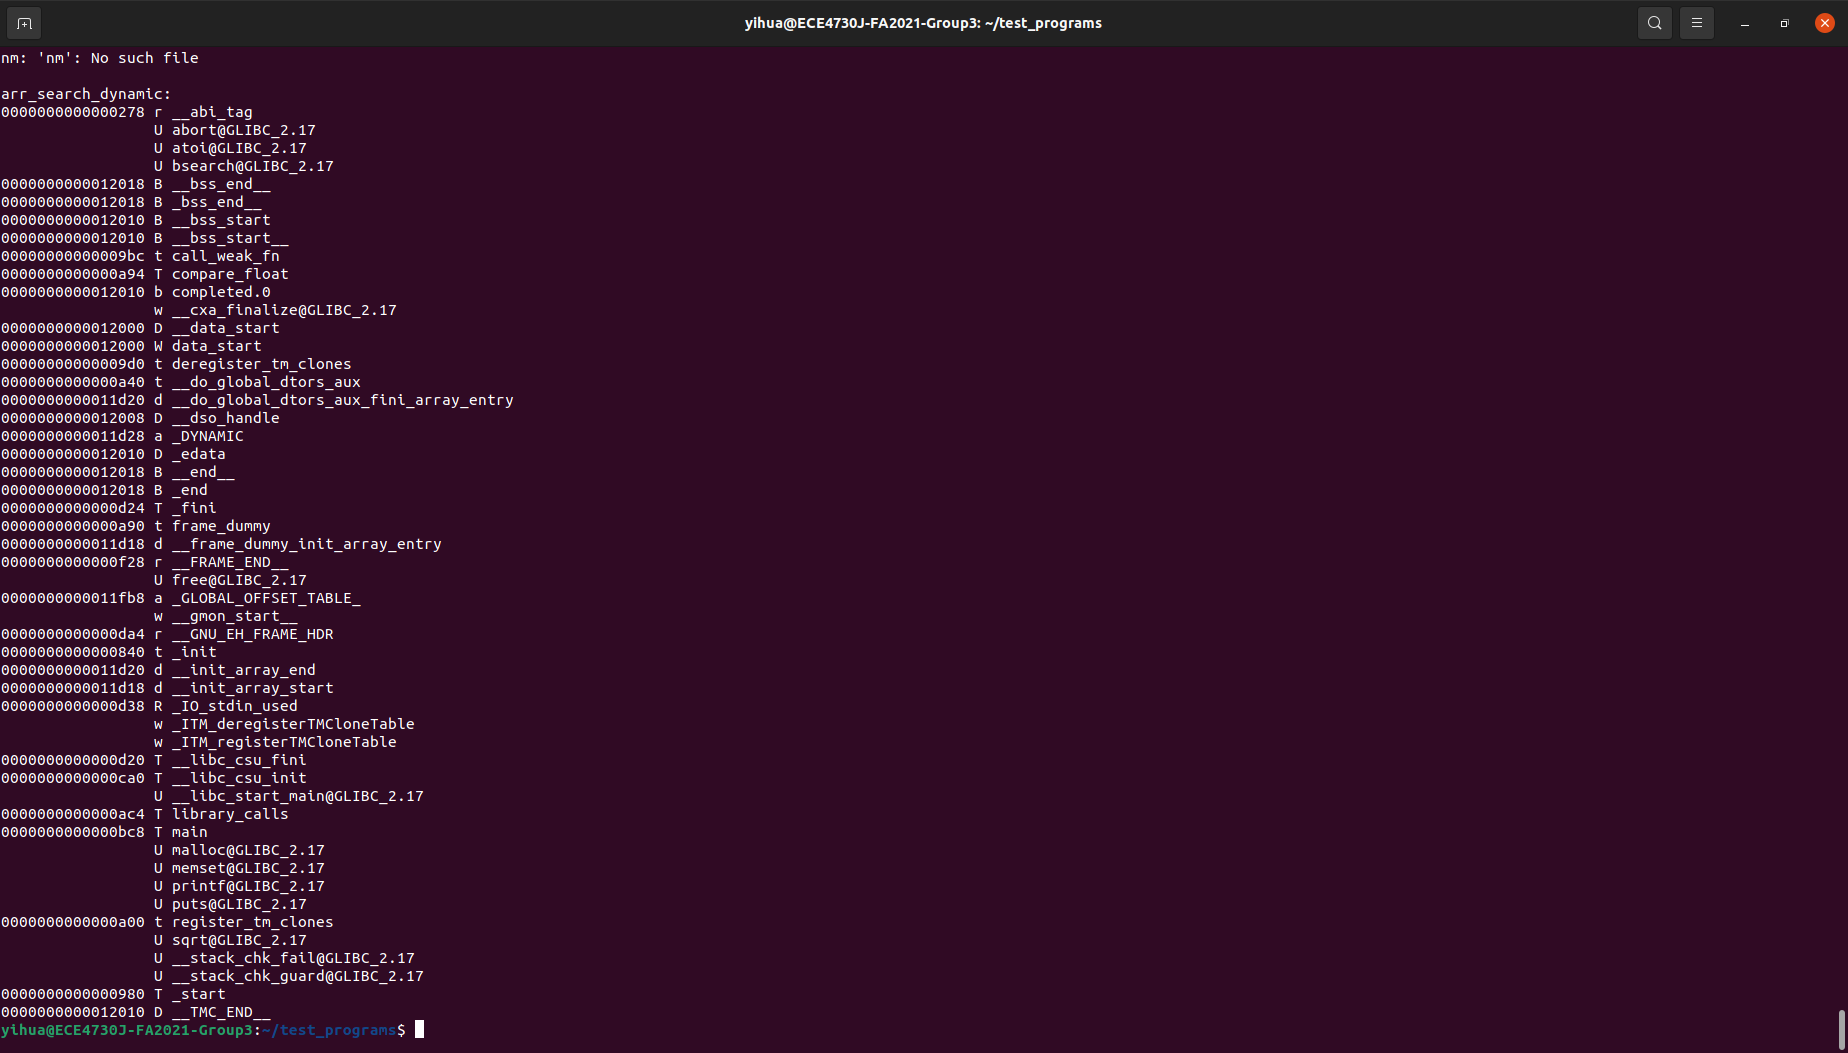
\includegraphics[width=1\textwidth]{5.png}
    \caption{\texttt{nm} command (dynamic).}
\end{figure}
\texttt{nm} command is used to list symbols from object files. The statically compiled program has a lot of symbols, and all the symbols of library code are listed, such as \texttt{malloc} of \texttt{stdlib.h} and \texttt{strchr} of \texttt{string.h}, while the dynamically compiled program has relatively less symbols.

6.
\begin{figure}[H]
    \centering
    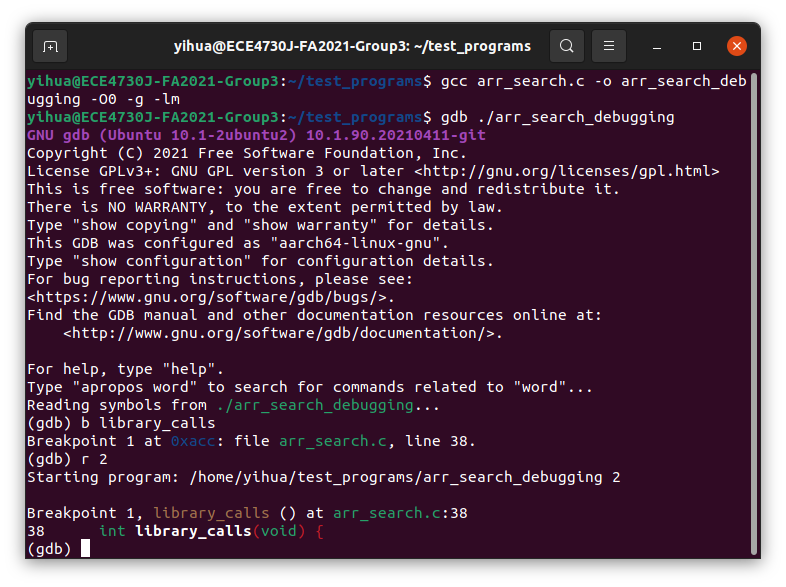
\includegraphics[width=1\textwidth]{6.png}
    \caption{Compiling and loading programs by \texttt{gdb}.}
\end{figure}
Using \texttt{-g} option to compile our program by \texttt{gcc} we can use \texttt{gdb} to debug.

7. \texttt{b} command adds a breakpoint, where \texttt{library\_calls} is the function. \texttt{r} commands runs the program, and 2 is the number of iterations.

8.
\begin{figure}[H]
    \centering
    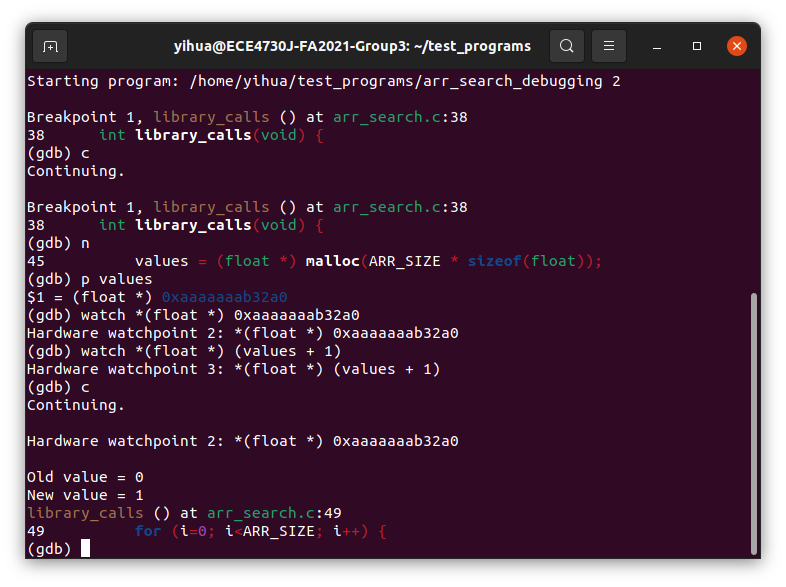
\includegraphics[width=1\textwidth]{7.png}
    \caption{Executing the program in \texttt{gdb}.}
\end{figure}
\texttt{c} command continues to the next breakpoint, and we can see that the program stops again at the function \texttt{library\_calls}, which indicates that we are executing the second time.

9. We can see that the address of the variable \texttt{values} is 0xaaaaaaab32a0.

10.
\begin{figure}[H]
    \centering
    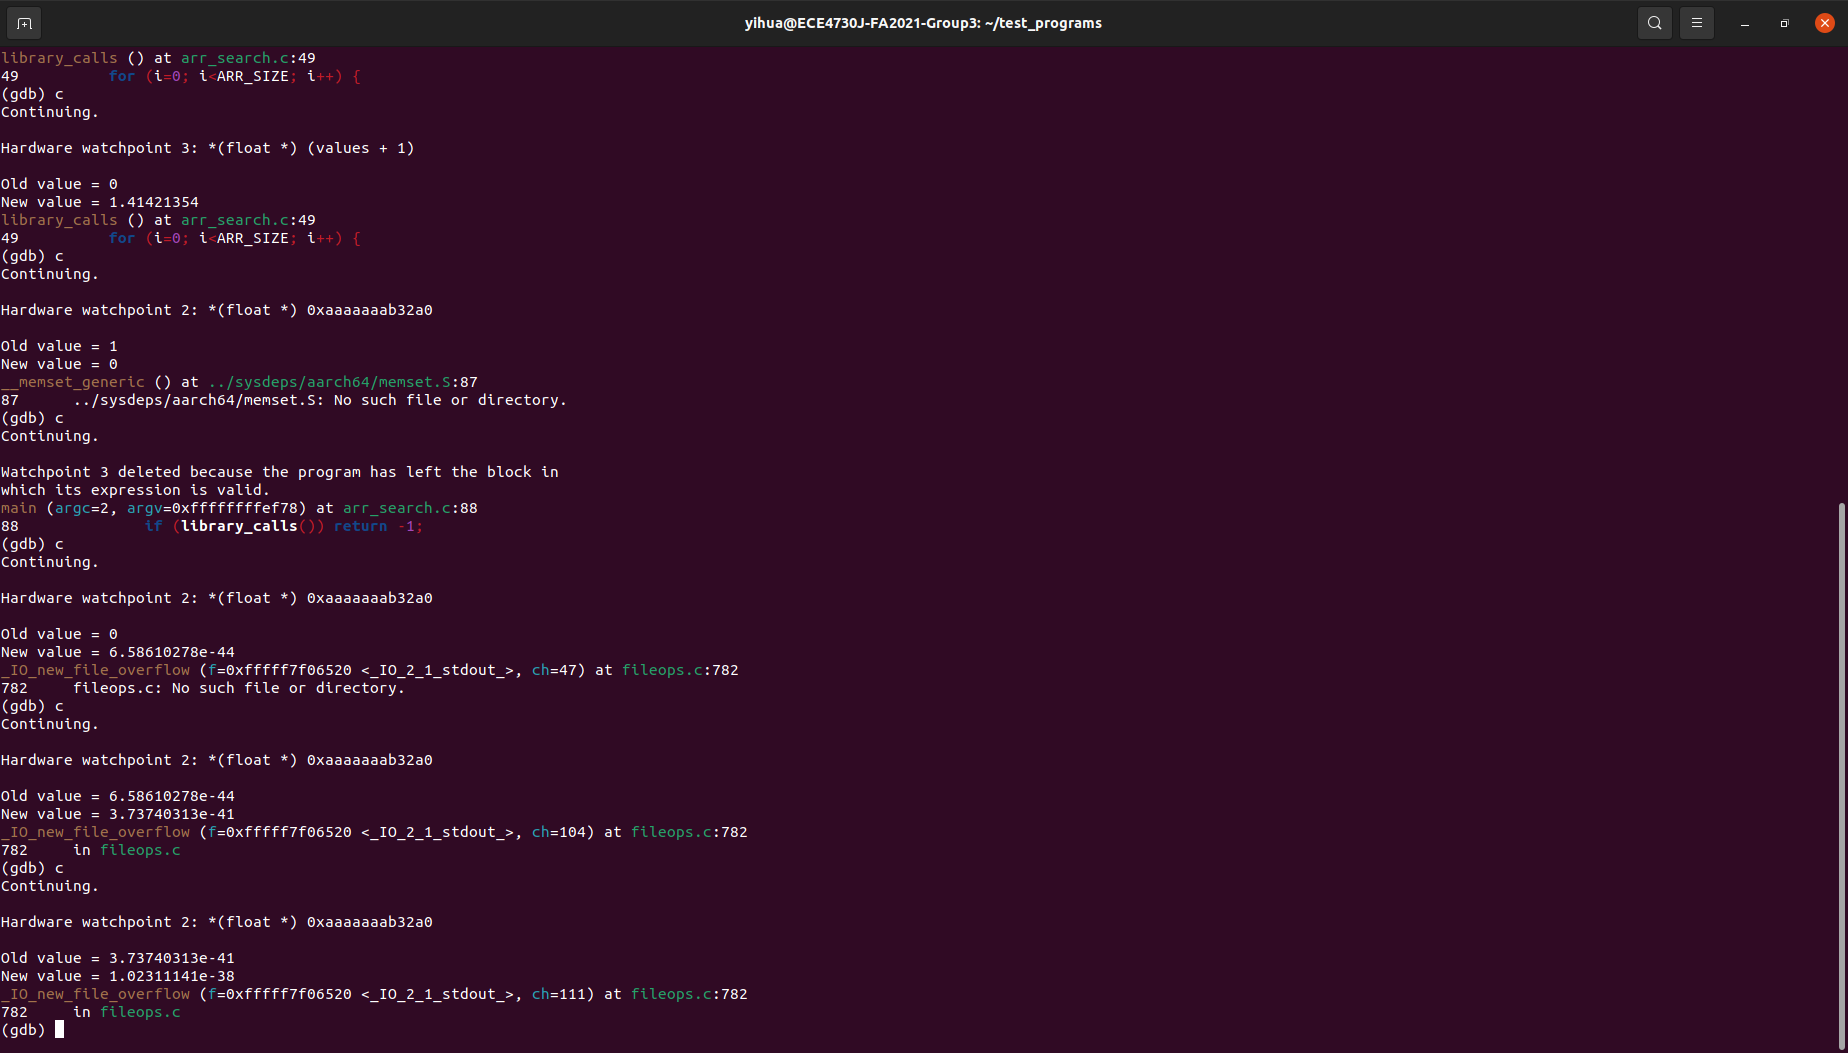
\includegraphics[width=1\textwidth]{8.png}
    \caption{Continue execution until the program execution exits.}
\end{figure}
\begin{figure}[H]
    \centering
    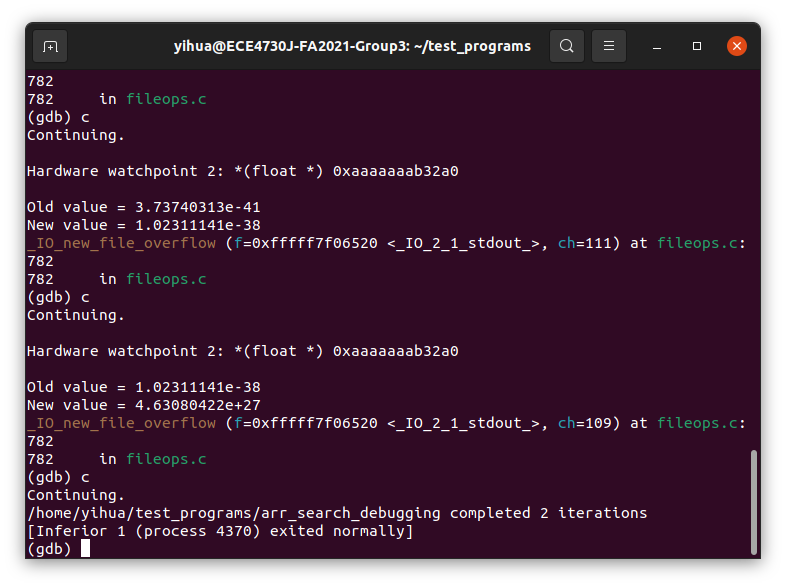
\includegraphics[width=1\textwidth]{9.png}
    \caption{Continue execution until the program execution exits.}
\end{figure}
Values of \texttt{values[0]}: $0\ ->\ 1\ ->\ 0\ ->\ 6.58610278e-44\ ->\ 3.73740313e-41\ ->\ 1.02311141e-38\ ->\ 4.63080422e+27$

Values of \texttt{values[1]}: $0\ ->\ 1.41421354$
\end{document}